% !TeX root=../main.tex

\begin{figure}[!t]
	\hspace*{-4cm}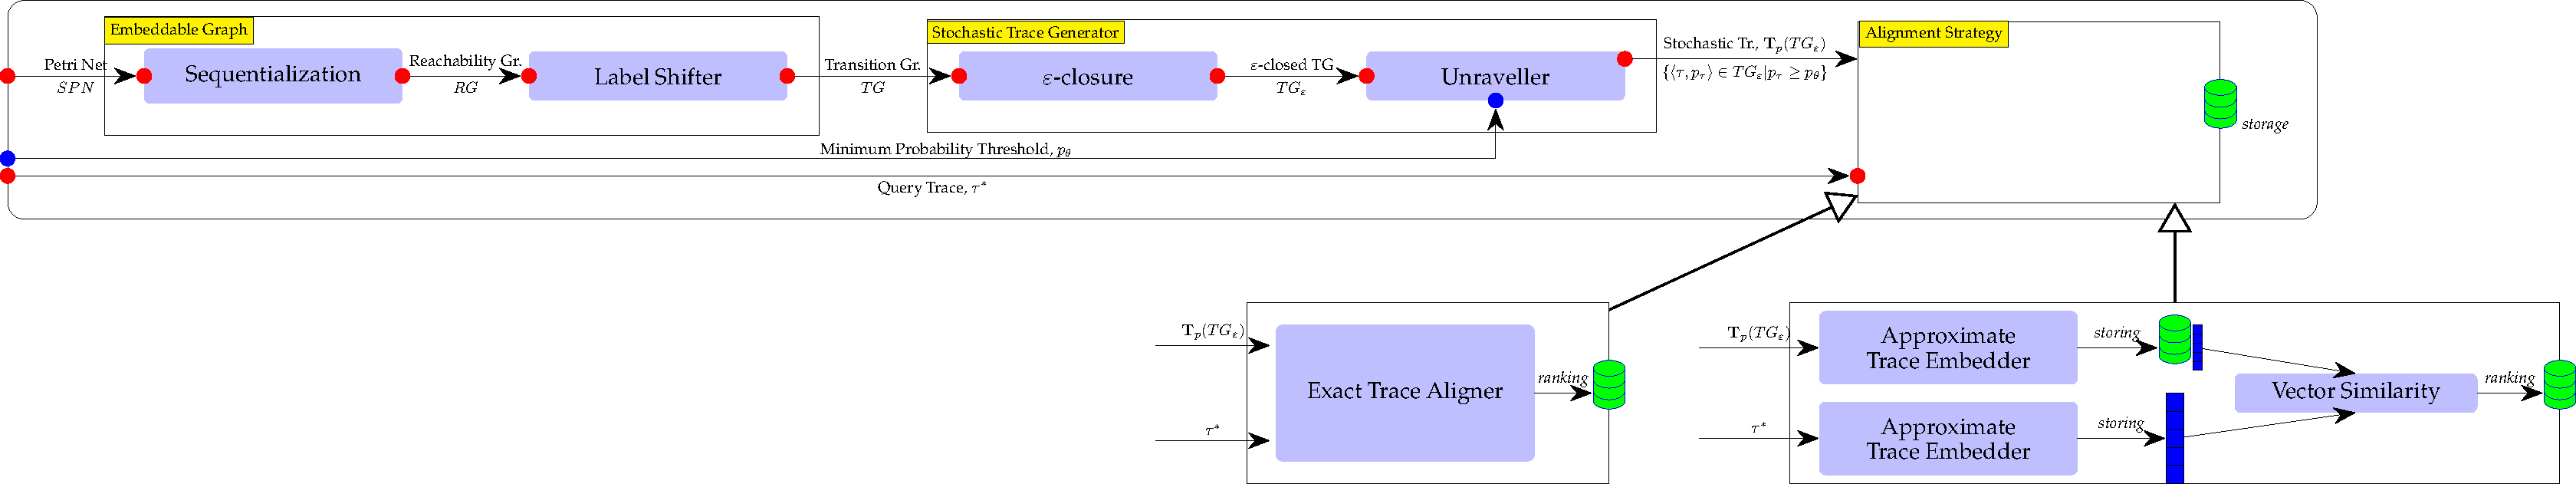
\includegraphics[width=1.7\textwidth]{images/pipeline}
	\caption{Proposed pipeline to assess the Probabilistic Trace Alignment}\label{fig:pipe}
\end{figure}


\section{Probabilistic Trace Alignment Pipeline}
We propose the pipeline from Figure \ref{fig:pipe} connecting several existing formalisations via intermediate processing steps. 
The input of this pipeline is a query trace to be aligned, an USWN, and a minimum probability threshold $p_\theta$. Its output 
is a set of model traces satisfying $p_\theta$ with an alignment ranking.
%
The pipeline has the following phases: after representing the USWN as a graph of all the sequentially scheduled transitions 
(\S\ref{sec:seqZ}), we shift the labels from the edges towards the nodes while preserving the set of probabilistic traces 
(\S\ref{sec:LSift}) and minimize the graph representation by removing the $\varepsilon$-labelled nodes while preserving the 
trace probability (\S\ref{sec:clos}). We extract the set of all traces having probability above $p_\theta$ threshold (\S\ref{sec:unrav}) and  apply two different alignment strategies; one exact  (\S\ref{subsec:eta}), and one approximated. 


We later discuss how to rank traces in the exact and approximated scenarios by reducing the alignment process to a k-nearest 
neighbour problem. While the exact trace alignment requires to perform the alignment process each time a novel trace $\tau^*$ is 
introduced (\S\ref{subsec:exbkptap}), the approximated alignment can split the alignment into a preliminary loading phase and a 
query phase. In the former, each stochastic trace from the USWN is represented as a vector (\S\ref{subsec:ate}), and in the latter the to-be-aligned trace $\tau^*$ is first represented as a vector and then compared to all the other vectorial representations.  

\subsection{Sequentialization}\label{sec:seqZ}
The sequentialization step transforms a USWN with an initial marking $M$ into a Reachability Graph $(\mathcal{M},\mathcal{E})$ 
generated by a sequentialization process, where potentially concurrent firing transitions are represented via a sequential scheduling. 

\begin{definition}[Reachability Graph]
	Given an initial marking $M$ for a USWN $\mathcal{U}$,  the \textit{Reachability Graph} for $\mathcal{U}$ is a graph 
	$(\mathcal{M},\mathcal{E})$ where the nodes  $\mathcal{M}$ are composed of all the reachable markings from $M$, 
	and the edges $\mathcal{E}$ are induced by the aforementioned relation $M\overset{t}{\to}M'$ among the 
	nodes. To each edge $M\overset{t}{\to}M'$, we associate a transition probability $\mathbb{P}\left(M\overset{t}{\to}M'\right)=\frac{W(t)}{\sum_{t'\in E(M)}W(t')}$ \cite{spdwe}. 
\end{definition}

\begin{example}
From the USWN in Figure \ref{fig:spn}, the sequentialization process generates the reachability graph depicted in 
Figure \ref{fig:rg}. Each node represents a marking $M$ as a vector, and the edges are labelled with the firing transitions. 
The edges associated to this graph describe potentially concurrent firing transitions sequentially. While visiting the graph from 
$M$, the chaining of the edge labels generates a trace produced from the Untimed Workflow Net, and the product of the edge 
weights provides the probability associated to the trace.
\end{example}



\subsection{Label Shifter}\label{sec:LSift}
Reachability graphs obtained via sequentialization cannot be directly embedded using existing methods:  Reachability graphs 
associated to stochastic workflow nets are edge labelled, but TGs are node labelled. To represent the former as the latter, we 
shift the labels from the edges to the nodes  while preserving the set of traces and their associated probability. 
Such transformation is defined next.

\begin{definition}[Label Shifter]\label{def:transf}
The reachability graph $(\mathcal{M},\mathcal{E})$ generated from an initial marking $M$, is transformed into the TG $(s,t,L,R,1)$, where:
\begin{itemize}
	\item If is a single edge $M_1\overset{t}{\to}M_2\in\mathcal{E}$ where $M_1=M$, then $s=M\overset{t}{\to}M_2$; otherwise, define a new node $\textbf{i}$ and set it as the initial node for TG: $s=\textbf{i}$.
	\item If is a single edge $M_1\overset{t}{\to}M_2\in\mathcal{E}$ without outgoing edges in the reachability graph, then $t=M_1\overset{t}{\to}M_2$; otherwise, define a new node $\textbf{f}$ and set it as the accepting node for TG:  $t=\textbf{f}$.
	\item $[L]_{\lambda(t),\;M\overset{t}{\to} M'}=1$ for each $M\overset{t}{\to} M'\in\mathcal{E}$; if $\textbf{i}$ is defined then $[L]_{\varepsilon\textbf{i}}=1$; if $\textbf{f}$ is defined, then $[L]_{\varepsilon\textbf{f}}=1$; $[L]_{ij}=0$ otherwise.
	\item $[R]_{M\overset{t}{\to} M',\;M'\overset{t'}{\to} M''}=\frac{W(t')}{\sum_{\textbf{t}\in E(M')}W(\textbf{t})}$ for each $M\overset{t}{\to} M',M'\overset{t'}{\to} M''\in\mathcal{E}$; if $\textbf{i}$ is defined, $[R]_{\textbf{i},\;M\overset{t}{\to}M'}=\frac{W(t)}{\sum_{\textbf{t}\in E(M)}W(\textbf{t})}$; if $\textbf{f}$ is defined, then $[R]_{M\overset{t}{\to}M',\;\textbf{i}}=1$ for each $M'$ without outgoing edges in the reachability graph; $[R]_{ij}=0$ ow.
\end{itemize}
\end{definition}
%
We can show that the TG obtained in Definition \ref{def:transf} preserves the same set of probabilistic traces associated by the reachability graph. The proof is omitted due to the lack of space.

\begin{example}
Figure \ref{fig:lmc} provides the output of such transformation if Figure \ref{fig:rg} is used as an input. All the nodes are labelled using the firing transitions' labels (in green), while the edges preserve the probabilistic information from the Reachability Graph (in red). Intuitively, when a new initial node \textit{\textbf{i}} is inserted, we preserve all the initial probabilistic choices that a transition is fired from an initial marking $M$, while all the intermediate edges inherit the probabilisitc choice of the firing transition from the subsequent choices. When a new final node \textit{\textbf{f}} is added, such edges always have probability $1$, and therefore we do not interfere with the initial traces' probability.
\end{example}

\subsection{$\varepsilon$-closure}\label{sec:clos}
The $\varepsilon$-closure process has two main purposes: first, it reduces the size of the Transition Graph generated in the previous step by removing all the $\varepsilon$-labelled nodes \texttt{\color{blue}w} and preserving the connection between  the nodes \texttt{\color{blue}u} from its ingoing edges   $\texttt{\color{blue}u}\xrightarrow{\color{red}p_i}\texttt{\color{blue}w}$ with the nodes \texttt{\color{blue}v} from its ingoing edges   $\texttt{\color{blue}w}\xrightarrow{\color{red}p_j}\texttt{\color{blue}v}$ by establishing new edges $\texttt{\color{blue}u}\xrightarrow{\color{red}p_ip_j}\texttt{\color{blue}v}$. $\varepsilon$-labelled initial (or accepting) nodes are removed if and only if they have only one outgoing (ingoing) edge with probability $1$.

\begin{example}
	The $\varepsilon$-closure remotes the non-initial and non-accepting nodes within such automaton, while preserving the probabilistic trace equivalence of the two automata: node \texttt{\color{blue}10} is then removed alongside its associated edges, and new edges $\texttt{\color{blue}3}\xrightarrow{\color{red}p_4}\texttt{\color{blue}4}$ and $\texttt{\color{blue}3}\xrightarrow{\color{red}p_5}\texttt{\color{blue}5}$ are introduced. The resulting TG $P$ is represented with the same graphical depiction Figure \ref{fig:closed}.
\end{example}

Consequently, it is always possible to minimize a TG  (e.g., Figure \ref{fig:orig}) via $\varepsilon$-closure, so that the only nodes that are labelled as $\varepsilon$ are the source and the target nodes (Figure \ref{fig:closed}) and the set of weighted traces is preserved. From now on, we always that all the TGs are minimized via $\varepsilon$-closure. 

\subsection{Unraveller}\label{sec:unrav}
Being that both the graph isomorphism problem is NP-Complete and the TGs are fully characterized by the set of the probabilistic traces that they generate,  we can say that two TGs are (probabilistic-trace) equivalent if and only if they share the same set of weighted traces. In particular, we denote as $\mathcal{W}_p^n(P)$ the set of all the weighted traces in $P$ having at least probability $p$ and maximum length $n$. Under these assumptions, the probabilistic trace equivalence is deterministic.

\begin{example}
	The TG in Figure \ref{fig:orig} has the following set $\mathcal{W}_0^{\aleph_0}(P^*)$ of weighted traces:
$$\set{\braket{\underbrace{\color{green}a\dots a}_{n},{\color{red}p_1p_3^np_6}}|n\in \mathbb{N}_{>0}}\cup \set{\braket{{\color{green}c}\underbrace{\color{green}a\dots a}_{n},{\color{red}p_2p_4p_3^np_6}}|n\in \mathbb{N}_{>0}}\cup\{\braket{{\color{green}cb},{\color{red}p_2p_5}}\}$$
After the $\varepsilon$-closure process, $\mathcal{W}_0^{\aleph_0}(P^*)=\mathcal{W}_0^{\aleph_0}(P)$, so the two TGs are (probabilistic-trace) equivalent.
\end{example}
